\documentclass{fisatproject}
\usepackage{graphicx}
\title{Website Design Ranking Using ML}
\team{Adhyaksh Guhan \\ Anet Eliza Johny\\ Dharwish Raj \\ Joel J Padayattil}
\author{Dharwish Raj}
\begin{document}
\maketitle

\makecert

\newpage
%\thispagestyle{plain}
\pagenumbering{roman}
\setcounter{page}{1}
\newgeometry{top=4cm,bottom=0.1cm}
\renewcommand\abstractname{ABSTRACT}
\begin{abstract}
\vspace{5cm}
This project attempts to review and rank websites objectively and without any human input. Most website design rankings,if not all, are subjective in nature and curated by human hands and minds.Website Design Ranker attempt to achieve similar results but with computer algorithms for a 	\item It must take into account various parts of the website to use as parameters.

\item for example: pepole won't be intrested to visit a site if they are berated with adds.Thus adds abo	\item It must take into account various parts of the website to use as parameters.

\item for example: pepole won't be intrested to visit a site if they are berated with adds.Thus adds above a degree will be considered as the parameter for ranking.

\item There are no existing algorithms or methods that manage to analyze and evaluate websites in this way.ve a degree will be considered as the parameter for ranking.

\item There are no existing algorithms or methods that manage to analyze and evaluate websites in this way.fairer comparison.

Website design ranking is usually done by a committee of experts or by mass voting on the internet. This method of ranking can be unfavorable due to the subjectivity of its nature.There are no clear standards on which everyone can definitely agree on and it causes the whole process to be an unfair popularity contest.This project,with its lack of human input and unbiased perspective can be used as an objective basis from where ranking can commence.

Currently,the ranking of the designs are done by the counting of the number of colours contained in a website. This is done by using a web scrapper to scrap the website and obtain the CSS file. The file is then parsed through using a regex method, and is used to find and count hexcodes contained within. The resulting number is then printed and then used as a parameter to rank-based on colour theory-if the website has too few colours or too many colours or if it has just the right amount.
\end{abstract}


\newpage
%\thispagestyle{plain}
\renewcommand\abstractname{ACKNOWLEDGMENT}
\begin{abstract}
\vspace{5cm}
If words are considered as symbols of approval and tokens of acknowledgement, then let the words play the heralding role of expressing our gratitude. Firstly, we praise the God Almighty for the grace he showered on us during our studies as well as our daily activities.

We thank our Principal,\textbf{Dr. George Issac}, for the amenities provided,which helped us in the fullfillment of our project. We would also thank our beloved \textbf{Dr. Prasad J.C. (H.O.D)} who helped in all the phases of our project.

We pay our gratitude to all project staff in-charges, \textbf{Ms. Soumya S. Raj, Mr. Anuranj P., Ms. Simi Stephen} for their constant support and encouragement for the project. We are extremely thankful to our project guide \textbf{Mr. Pankaj Kumar}, who always helped and guided for all the success of our project.

We express our sincere gratitude to all faculties of Computer Science Department, \textbf{FISAT}. We also thank our parents and friends for supporting in the completion of our project.
\vspace{1cm}
\begin{flushright}
Adhyaksh Guhan

Anet Eliza Johny

Dharwish Raj

Joel J Padayattil
\end{flushright}
\end{abstract}
\newpage

\restoregeometry
\tableofcontents
\newpage

\cleardoublepage
\addcontentsline{toc}{chapter}{\listfigurename}
\listoffigures
\newpage

\cleardoublepage
\addcontentsline{toc}{chapter}{\listtablename}
\listoftables
\newpage
\pagestyle{fancy}


\chapter{INTRODUCTION}
\pagenumbering{arabic}
\setcounter{page}{1}
\renewcommand{\baselinestretch}{1.50}
\section{Overview}
The website design is an important factor in the growth of that website. It makes a difference on how the target audience view the business or company. So website design ranking is important for the audience to choose the best website. Recently this ranking is done manually by looking into the websites by a group of people.

Ranking of website design manually is a difficult and time consuming method. Website Design Ranker can overcome this difficulty by automating the ranking mechanism. Since a perfect model for website ranking is not in practice this follows ranking according to submissions by critics. Website Design Ranker reduces the difficulty and increases the accuracy in ranking since it is using an algorithm for ranking.

Website Design Ranker will rank set of input websites based on certain parameters. Too many colors can create a sense of confusion. As colour is an important factor to attract as well as repel the audience of a website. So the Website Design Ranker uses colour as a parameter to rank different websites accordingly.
\section{Scope of Project}
There was no existing methodology for analyzing and evaluating website designs. The method which followed until this time was based on submissions by the critics. This method can be replaced by our automated system to rank website design based on the different parameters, say colour, grid etc.

Most subjective methods, like the current system of judgement based on the values of a group of individual critics, are unreliable as they are based on the biased aesthetic senses of each critic involved in the criticism. Such subjective systems are unreliable and unfair to all involved websites as they may or may not consider the various objective parameters of websites that actually makes each of them stand out from each other. This project aims to objectively judge a website's design based on these objective parameters and show a fairer way of judging website design so that the designer and audience understand what part of the website makes it appealing/unappealing.
\chapter{RELATED WORK}
\section{Google Page Layout Algorithm}
Google introduced Page Layout Algorithm to analyze website
readability.[1] It looks for the layout of the web page and the amount of
content we see in the page once we click on a result.[1] It focuses to reduce the difficulty of users to find the actual
content.[1]
The websites which does not have a lot of visible content
above-the-fold and dedicates a large fraction (above a normal
degree) to ads, will be affected.[1]


\begin{figure}
	
	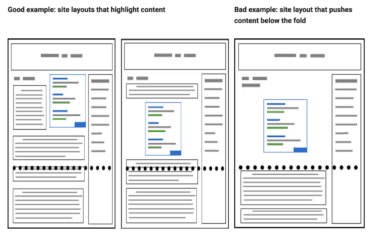
\includegraphics[width=10cm]{image/gpa.png}
	\caption{One of the criteria of GPL Algorithm\textsuperscript{[Fig:1]}}
	\label{fig1:gpa}
	
\end{figure}


Determine the old design of the website.If a website has many advertisements above the fold(the part of page that is visible on the screen when the page first loads before scrolling)then it is considered as the first drawback.Else if a website has a large flash animations or other
non-content elements that forces users to scroll to see the content, then that will be the next drawback. If there is specific amount of ads and content of website required for audience, there will be no drawback.These drawbacks will affect the ranking process. If these conditions are met the website ranks a low rank. Else its rank will be considerabily high.
\section{SEO Ranking}
SEO stands for Search Engine Optimization,which is  the practice of increasing the quality and quantity of traffic to websites through organic search engine results.
\begin{itemize}
	\item \textbf{Quality of traffic.}A website can attract all the visitors in the world, but if they're coming to the site because Google tells them that the website is  a resource for Apple computers when really the site is related to selling apples, that is not quality traffic. Instead it is to attract visitors who are genuinely interested in products that offer.
	\item \textbf{Quantity of traffic.}Once the right people clicking through from those search engine results pages (SERPs), more traffic is better.
	\item \textbf{Organic Results.}Ads make up a significant portion of many SERPs. Organic traffic is any traffic that don't have to pay for.
	
	Google(or any search engine) has a crawler that goes out and gathers information about all the content they can find on the Internet. The crawlers bring all those 1s and 0s back to the search engine to build an index. That index is then fed through an algorithm that tries to match all that data with your query.There are a lot of factors that go into a search engine's algorithm.
	The purpose of the page is to Expertise, authority, and trustworthiness – not just from the site and the page content, but expertise from the individual creator of the content too,Content quality and amount,Website info and info about the content creator,Website reputation and content creator reputation.\newline
	\newline
	The most important SEO ranking factors are:
	\item A Secure and Accessible Website
	\item Page Speed (Including Mobile Page Speed)
	\item Mobile Friendliness
	\item Domain Age, URL, and Authority
	\item Optimized Content
	\item Technical SEO
	\item User Experience
	\item Links
	\item Social Signals
	\item Real Business Information
	\newline
	\newline
	\newline
	\newline
	\newline
	\newline
\end{itemize}
The first of our SEO ranking factors has to do with having the right kind of URL. Specifically, that’s a URL that Google’s bots can easily reach and crawl.\newline
In other words, Google has to be able to visit the URL and look at the page content to start to understand what that page is about. Google announced a search engine algorithm update focused on mobile page speed that will start to affect sites from July 2018. If site doesn’t load fast on mobile devices, then it could be penalized.\newline
Things to look at  also include:
Whether this is a responsive site that automatically resizes to fit the device,
Whether it using large fonts for easy readability on a small screen,
Accessibility and navigability, including making it easy to tap menus,
Ensuring that essential content isn’t hidden by interstitial ads.\newline
One negative SEO ranking factor to be aware of is duplicate content. For SEO, fresh, original content is always best. And if it do have content that’s similar, tell Google which one should be ranked as most authoritative by using canonical URLs.
Getting the code right is one aspect of optimizing content for better search engine rankings.\newline Some of the aspects need to look are:
Use keyword phrases in page titles, which is where Google first looks to determine which content is relevant to which search. Will see the page title as the first line of a search result entry.
Use header tags to show content hierarchy. If title is formatted as h1, then use h2 or h3 for subheads.
Create a meta description that both entices readers and includes your keyword phrase. Keep meta descriptions short and grabby – it have right around 160 characters to convince searchers that this is the post they want.\newline
Use keyword phrases in image alt tags to show how the images are relevant to the main content. Google also has an image search, which is another way for people to find content.\newline
Where it’s appropriate, use schema markup to tell Google what kind of content is producing. This can also help content appear in rich card entries other than answer boxes.Optimize titles, descriptions, and content to get the clicks and deliver value on the other end,Thus boost search engine ranking.\newline
Google search results usually have a lot of shares – probably because more the content is shared, the more people will see it and decide to link to it. That means that getting more social shares does help the search engine rankings, if only indirectly.The presence or absence of business information is another crucial factor for local SEO ranking factors.



\section{CTA}

Click-through rate measures the number of people who click a link against the total number of people who had the opportunity to do so.It’s calculated by dividing the number of people who click after seeing the ad by the total number of impressions the ad received.
In other words, a high CTR means that it has targeted the right people, it had interesting copy and it had an offer that was appealing enough that a large percentage of ad viewers are clicking.This is an excellent sign.Conversely, a low CTR often means that ads are not a good match for target audience.


A blog is the best resource to connect with new website visitors and to keep returning visitors engaged.There are a few golden rules when it comes to a successful blog. CTAs (Calls To Action) are a must have.Without a CTA, customers who are interested in the products may not know what to do next. Instead of hoping they contact you, a CTA tells them what the next step is and invites them to take it.
\begin{figure}
	\vspace*{1cm}
	\hspace*{0.01cm}\includegraphics[width = 0.9 \linewidth]{click.png}\hspace*{-cm}
\end{figure}

\chapter{DESIGN and IMPLEMENTATION}

\section{Design}
The Website Design Ranker will rank a set of input websites based on certain parameters. The parameter this project mainly focuses on is colour.
The system requires an input: the URL of the corresponding website that needs to be ranked. Once the URLs have been pasted as input, each one is scraped to find their CSS files and count the hexcodes within them.
\begin{itemize}
	\item It is an HTTP request which is sent to the URL of a webpage that we
	are to access.
	\item The HTML contents are then parsed through using a parsing library
	found in Python, as the data is nested.
	\item The HTML contents are then parsed through using a parsing library
	found in Python, as the data is nested.
	\item \textbf{Beautiful Soup}, the library responsible for parsing, allows our created
	\textbf{Regular Expression} to search through the extracted data and find
	the hexcodes.
	\item After counting the number of colours, an appropriate score will be
	assigned to the corresponding website using colour theory—i.e, too many
	and fewer colours earn less marks, while good use of colour earns more.
	\item The ranking data is based on a conducted user survey to assess the
	overall appeal of a website’s design (from 1 to 5 stars).
\end{itemize}

In order to help achieve an objective rank parameter for the colours, a public review website was created via PHP hosted on an apache server. Survey participants were given a list of websites' frontpage, each of which could be rated from 1-5 stars (1 being the lowest and 5 being the highest).
After the survey was completed, the results were aggregated to be taken as the rank parameter for the program.
This will be helpful in finding the best website among list of websites as the website's design can be compared with the other competing websites.

Hence, this shows where a  website’s design can improve in an area and how it stacks up against other websites.


\subsection{Algorithm}
\begin{itemize}
	\item[1.] Start.
	\item[2.] Using a website scraper to accept the various website
	addresses.
	\item[3.] Scraping through the source code of each website via CSS files.
	\item[4.] Find the hex codes of all elements of the website and count them with a count variable.
	\item[5.] If count == 0 then give mark as 0.
	\item[6.] else if count is greater than or equal to 5, then also give mark as 0.
	\item[7.]If the count is less than or equal to 5,then the mark provided will be 1.
	\item[8.]Stop.
\end{itemize}
\subsection{System Requirements}
\subsubsection{\underline{Software Requirements}}
\begin{itemize}
	\item Operating System : LINUX OS 
	
	\item Language : Python
\end{itemize}

\subsubsection{\underline{Hardware Requirements}}
\begin{itemize}
	\item Processor : Intel Core i3 
	\item RAM : 4 GB
	\item Hard Disk : 128 GB
	
\end{itemize}


\section{Implementation}
\subsection{Data Flow Diagram - Level 0}
\begin{flushleft}
	\centerline{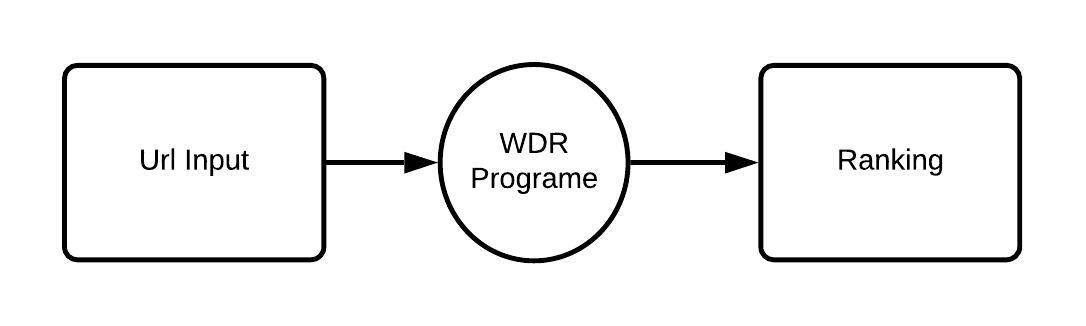
\includegraphics[scale=1.2]{image/level_0_dfd.jpeg}}
\end{flushleft}

On the basis of colour theory, we count the number of colours to determine the ranking of the website.
Too few colours, then the website is extremely simple and too boring.
Too many colours, then the website is over-designed and busy.

The system works by scrapping CSS file of different websites using webscrapper and from that CSS files it find and count the hexcodes of websites using regular expression. This count is used to rank the websites accordingly. Websites with too many and too few colours are ranked less and those with a specific count of colours are ranked high.  
  \subsection{Webscraping using Beautifulsoap}
  \begin{itemize}
 \item It is an HTTP request which is sent to the URL of webpage that we are to access. In return the server respont by returning HTML contents. Here a third party library is used for the requests.
 \item When we access the HTML contents, then we move to the task of parsing data. As the HTML data is nested one need a parser.
 \item Many HTML parser libraries are available, but the most advanced is html5lib.
 \item Now, the created Parse Tree is navigated. For this, another third party Python Library, Beautiful Soup, is used. It is a Python library for extracting data from HTML and XML files.
  \end{itemize}
	\subsection{Website Design Survey using PHP}
	\begin{itemize}
		\item In order to create a reasonable rank parameter, data was needed to justify and inform its use.
		\item As such, a survey was created where the participant pool was large enough such that, an accurate aggregate of data could be extrapolated
		\item The survey itself was created using php and was hosted as a website where participants would be shown screenshots of the main page of certain websites and then asked to rank from 1 to 5 stars.
		\item After the survey was completed, the aggregate of the end rankings of the highest ranked websites were used as the rank parameter for the main website design ranker.
	\end{itemize}	
\chapter{TESTING}

	Testing was done in several stages of this project. It was helpful to determine suitable language and library to collect data from different websites to find out ranking\\
	\subsection{Scrapping CSS codes from websites}
\begin{itemize}
	\item A website template's 'style.css' file was downloaded and then used as subject to testing the colour counting code.
	\item A website was created to have public ranking of various websites with a possible ranking of 1-5 (1 being the lowest, 5 the highest). This could then be used as ranking data for the program.
\end{itemize}
	\subsection{Website Survey using PHP}
	\begin{figure}[h]
		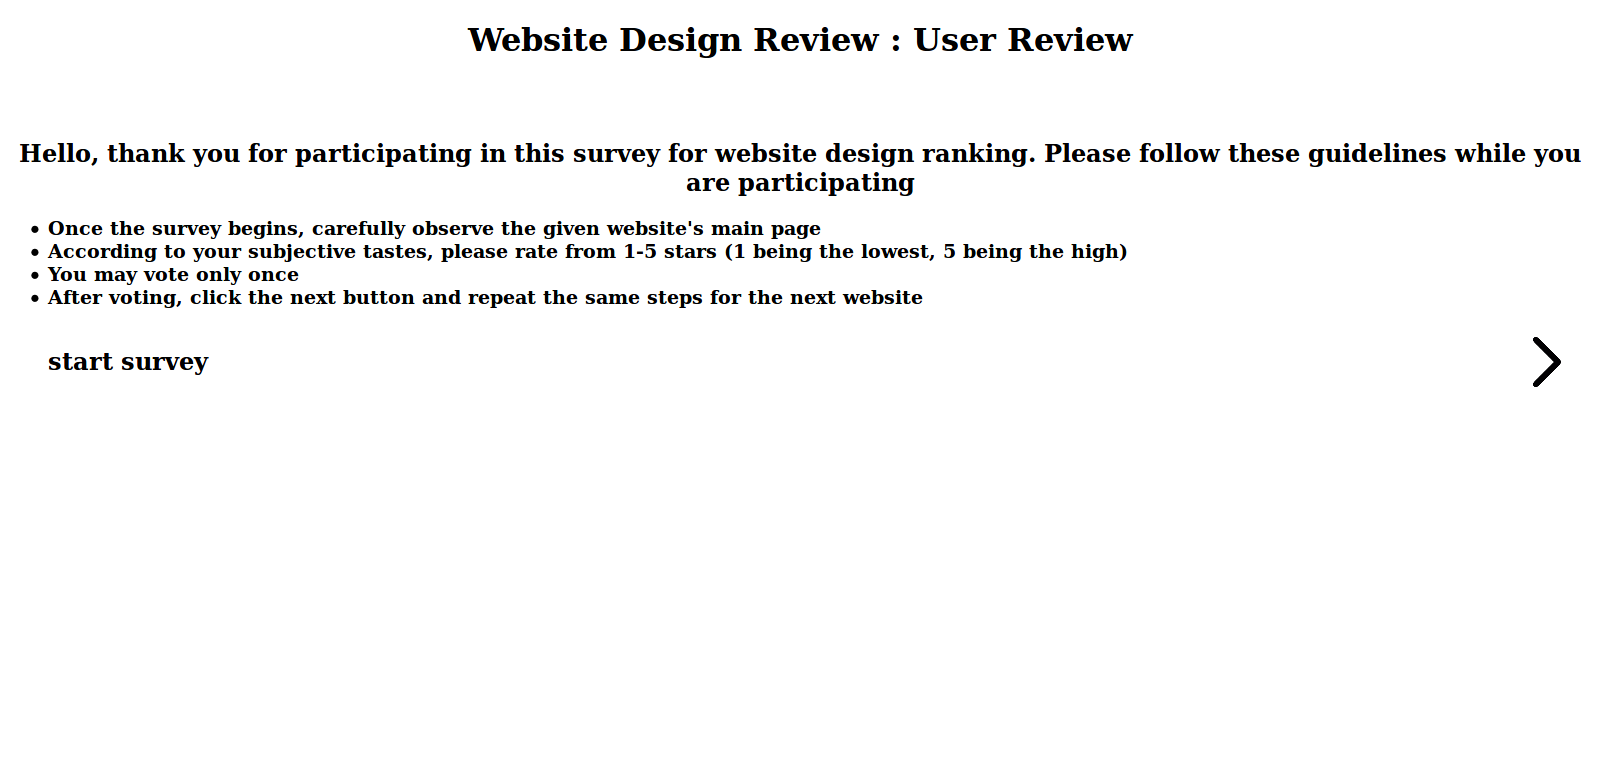
\includegraphics[scale=.25]{surveyrank.png}
	\end{figure}
	\begin{itemize}
		\item The survey was designed such that each person could only vote for each website once and then move on to the next one until it was complete.
		\item Each participant was asked to vote based on their own subjective tastes. This would be counterintuitive if it were not for the large participation pool from where the aggregate data could be extrapolated.
	\end{itemize}
	\chapter{RESULTS}
	\begin{itemize}
		\item Number of colours counted:
	\begin{figure}[h]
		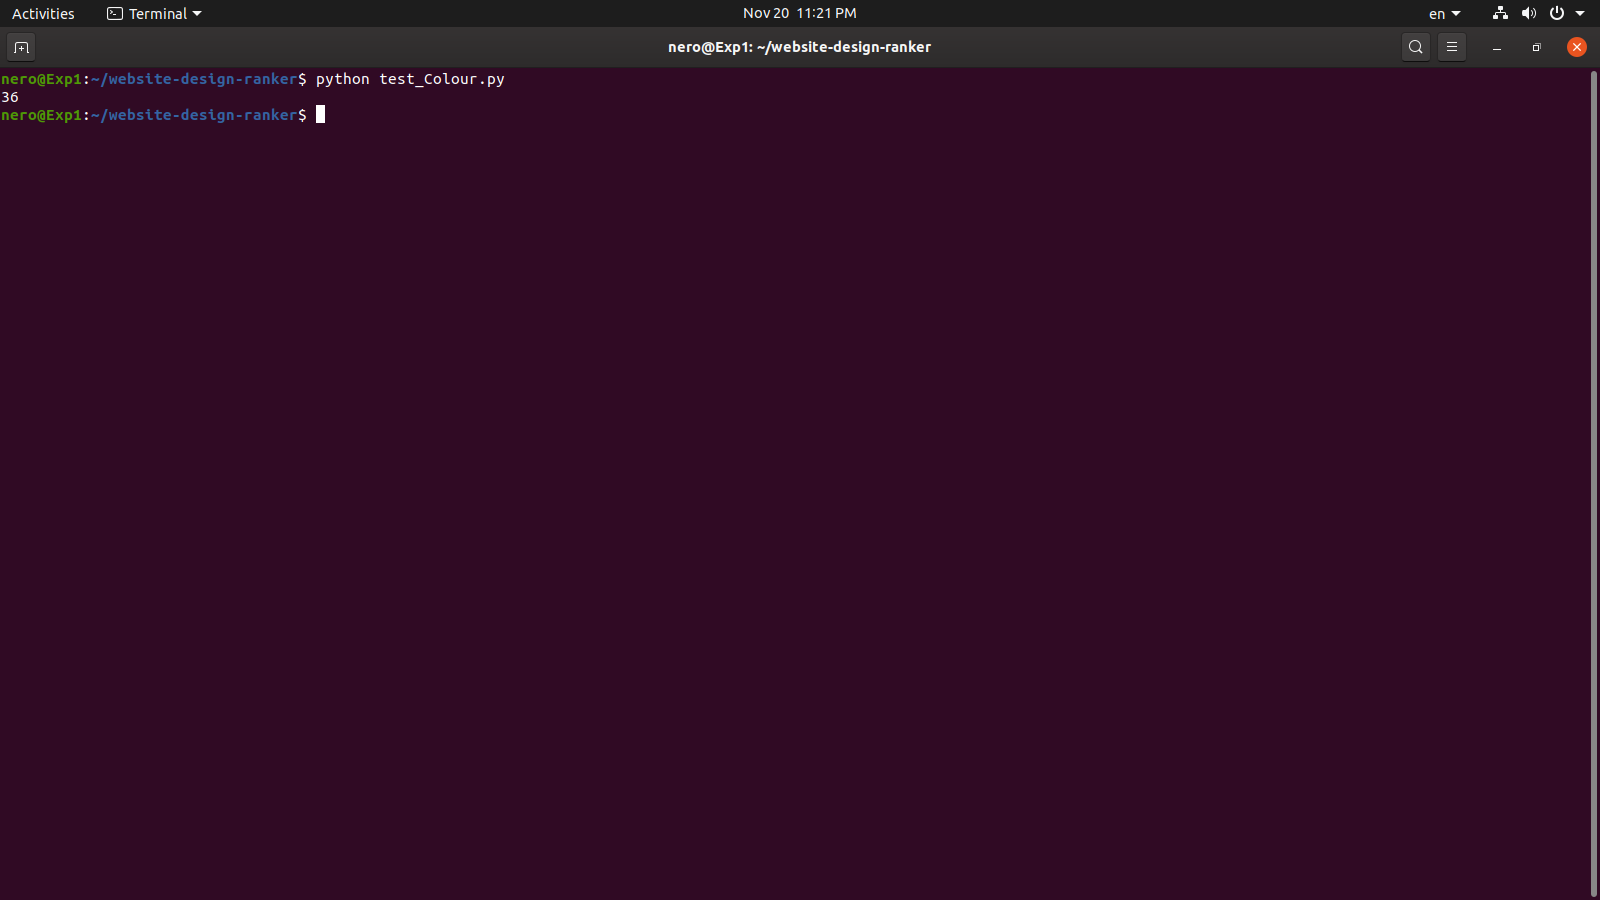
\includegraphics[scale=.3]{colourtest.png}
	\end{figure}
	\end{itemize}

\chapter{CONTRIBUTIONS}
\begin{itemize}
	\item Dharwish Raj - Creation of website for public ranking and code correction
	\item Adhyaksh Guhan - Creation of code for colour counting and spell checking
	\item Joel J Padayattil - Creation of UI using PyQT5
	\item Anet Eliza Johny - Proposed and Implemented basic algorithm 
\end{itemize}
\chapter{CONCLUSION}

A Website Design Ranker is an automated method to rank websites based on their design by comparing certain parameters. Here we can see the logical differences in the approaches that our algorithm takes versus any existing methods.To make ranking easier, the Website Design Ranker uses an algorithm to rank websites based on parameter colour.

Nowadays, ranking websites is done manually by a committee or a group of people. To avoid or to reduce the human involvement, Website Design Ranker is a suitable method. In this report, we have discussed our approach to rank a website design.



\begin{thebibliography}{1}
\bibitem{nist} Google Page Layout Algorithm: Everything You Need to
Know
 \url{https://www.searchenginejournal.com/google-algorithm-history/page-layout/close}

\end{thebibliography}

\begin{appendices}
\chapter{Sample Code}
\begin{lstlisting}[language=python]
	import re
	with open('style.css') as f:
	file\_contents = f.read()
	regex = r':?.(\#[0-9a-fA-F]\{6\}|\#[0-9a-fA-F]\{3\})'
	result = re.findall(regex, file\_contents)
	print(len(set(result)))

\end{lstlisting}
\end{appendices}


\end{document}
